\section{Decoder alternatives and posterior sampling}

\subsection{Alternatives that did not replace the selected PnP solver}

\par\medskip\noindent\begin{minipage}{\linewidth}
\captionof{table}{Alternative reconstruction directions and why they were not adopted.}
\centering
\begin{tabular}{@{}>{\raggedright\arraybackslash}p{0.313333\linewidth}@{\hspace{0.03\linewidth}}>{\raggedright\arraybackslash}p{0.313333\linewidth}@{\hspace{0.03\linewidth}}>{\raggedright\arraybackslash}p{0.313333\linewidth}@{}}\toprule
Direction & Observation & Conclusion for this study \\
\midrule
Generic DnCNN variants & 17L/17H/non-blind 17N did not improve the validation result & Changing generic noise variants was not sufficient. \\
Explicit non-negativity & Approximately baseline; iterates were already largely non-negative & No useful additional gain. \\
BM4D hybrid & Small validation gains, about 0.1--0.2 dB & A useful volumetric-prior clue, but not the best decoder. \\
Learned 2D or 3D alone & Smaller or inconsistent improvements & Combining learned slice and volume branches was stronger. \\
3D U-Net branch & Better standalone denoising, slightly worse PnP recovery & Denoiser quality alone did not rank inverse-problem performance. \\
Annealed non-blind HQS & No improvement over the selected solver & Not adopted. \\
MoDL-style unrolled 3D network & Two runs plateaued near 26 dB validation; output weakly depended on measurement count & Behaviour consistent with prior domination in this implementation, not a general failure of unrolling. \\
More ADMM iterations & 100 iterations performed worse than 20 in the screen & Extra iteration count did not solve the compressed-recovery problem. \\
Independent random plate for every image & An acquisition oracle gained only about 0.15--0.45 dB in the partial validation screen & Removing the fixed-plate constraint offered little improvement in that test. \\
\bottomrule\end{tabular}
\end{minipage}\par\medskip


The MoDL experiment was checked with both fine-model and coarse-basis measurements. Similar performance in both cases argued against discretisation mismatch as the main cause of its failure. It therefore remained a decoder-training or measurement-use problem to investigate, rather than a reason to change the optical model. The tested alternatives were not adopted; their outcomes do not establish universal method rankings.

\subsection{GPnP: estimation and uncertainty are different questions}

Generative PnP was implemented as an annealed split-Gibbs sampler with non-blind 2D/3D denoisers and a perturb-and-optimise likelihood update using the stated noise scale. Sixteen chains were used for the final posterior-mean and uncertainty summaries. Its settings were calibrated on validation data for nominal 90\% foreground coverage.

\par\medskip\noindent\begin{minipage}{\linewidth}
\captionof{table}{GPnP estimation and foreground uncertainty; final eight-subvolume aggregation.}
\centering
\begin{tabular}{@{}>{\raggedright\arraybackslash}p{0.176000\linewidth}@{\hspace{0.03\linewidth}}>{\raggedright\arraybackslash}p{0.176000\linewidth}@{\hspace{0.03\linewidth}}>{\raggedright\arraybackslash}p{0.176000\linewidth}@{\hspace{0.03\linewidth}}>{\raggedright\arraybackslash}p{0.176000\linewidth}@{\hspace{0.03\linewidth}}>{\raggedright\arraybackslash}p{0.176000\linewidth}@{}}\toprule
Images & GPnP mean PSNR (dB) & GPnP depth (\ensuremath{\mu}m) & Learned PnP PSNR (dB) & 90\% foreground coverage \\
\midrule
256 & 33.11 & 0.363 & 33.20 & 0.606 \\
64 & 26.93 & 0.785 & 32.69 & 0.807 \\
32 & 26.19 & 0.903 & 32.11 & 0.782 \\
16 & 23.88 & 1.066 & 31.13 & 0.766 \\
\bottomrule\end{tabular}
\end{minipage}\par\medskip


At full measurements its mean estimate approached deterministic learned PnP, but compressed estimates were substantially worse. Predictive standard deviation correlated with absolute error at about 0.49--0.66, so the uncertainty maps contained useful information about where errors occurred. Their scale was less reliable: foreground intervals under-covered the reference, and the 16-image calibration selected the upper edge of its scale grid. High whole-volume coverage at some compressed settings did not imply good foreground calibration because most voxels were background.

\textbf{Conclusion:} GPnP did not improve compression in the tested implementation. It remains an uncertainty-analysis side result rather than the preferred estimator, and its intervals should not be treated as calibrated confidence statements.

Evidence: D23/D26; {\small\texttt{solver\_\allowbreak{}learned/\allowbreak{}}} screening logs; final GPnP block and {\small\texttt{tables/\allowbreak{}gpnp\_\allowbreak{}uncertainty.\allowbreak{}csv}}. The final eight-subvolume aggregation supersedes early ten-crop summaries that included showcase volumes.


\begin{figure}[htbp]
\centering
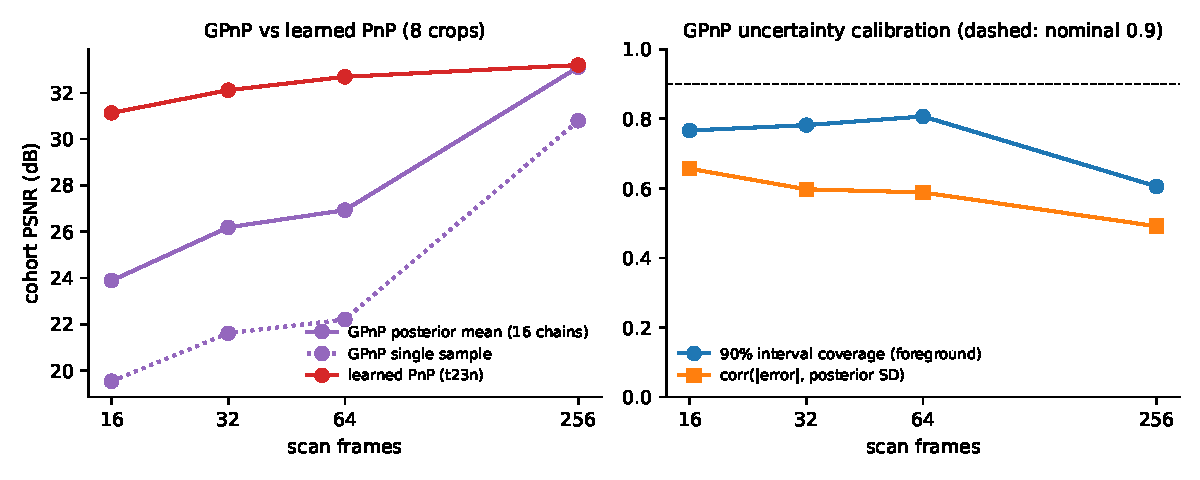
\includegraphics[width=\linewidth,height=0.48\textheight,keepaspectratio]{figures/generative_prior.pdf}
\caption{GPnP estimation and uncertainty. Posterior means deteriorate under compression, while nominal 90\% foreground intervals under-cover the reference. Original final-package plot; sixteen chains and eight test subvolumes.}
\label{exp:fig_gpnp}
\end{figure}
\FloatBarrier
